已经公布、但迄今尚未得到常规生产应用的一些成像概念均集中于本书这最后一章。本
章第一部分是建立线性时差的数学概念以及如何使它与速度分析联系起来。数据可以聚焦,
使得层速度可以直接读出。本章的后面部分是关于多次反射的讨论,线性时差在此处也有助
于明确问题。你将会孴到有能力处理多次反射及横向速度变化的基本数学工具。本章有许多
关于数据处理的建议,它们可不是那些生产过程的描述!

\section{地震资料解释}
\label{sec:5.0.1}

我最初把本章看作是适合于兴趣主要在于设计新型处理的专家。后来我认识到了在论述
似乎并不像所期望那样起作用的事情时,我们实际上首先要努力向现实作斗争,而不是为理
论预言而斗争。这一章对于熟练的解释人员来说将是有趣的。

石油勘探的核心问题是反射地震资料的解释。什么是地震解释?作为一位“按惯例办
事的解释员”,你必须通晓理论与实践普遍一致的任何事情;作为-一位好的解释员,你必须
知晓具有相似影响的交错变化现象之“噪音水平”。地震资料中的异常可能来源于地层本身
的复杂性、来源于地震波在地层内的传播(深层的、近地面的或射线平面以外的原因),或
者来温于记录系统和成像技术的不完善性。想在如此广泛的一种领域内做出清醒现实的判
断,你必须是这样一位地震学家:既是地质学家、又是工程师,同时还是数学家。本章不会
教你成为好的解释员,但是它将给你提供一次机会去评述若干关于地震理论与地震数据之关
系的批判性思路。

\subsection{倾斜}
\label{sec:5.0.2}

反射延迟时间非常类似于深度。我们通常是按偏离垂直射线的程度来测量角度,同时在实
际情形下也很少可能去记录零炮检距资料,最佳地震资料一般是远离垂直射线的。本章发展
建立了一种着重于某类特定选出之非垂直射的思路模式。坐标旋转解决不了这个问题,因
为旋转之后,将在其上进行观测的平面不会再直接位于$z=0$,旋转还会因形成某种很难对
付的二维函数$v'(x',z')$而把原来很简单的地震速度函数$v(z)$搞得一团糟。第三章中所
提出的炮检距观点也许看似相当完整,其实它并不十分全面,因为平方根是围绕垂直射线展
开的。\ref{sec:4.5}节建立的Stolt拉伸延展法曾阐述过丢下双曲线顶点不管而在两翼上进行拟合的好
处。

线性时差校正(LMO)是使人们重新认识我们关于非垂直射线这种思路的途径。尽管
尚未广泛被现代生产所吸收,这种较深刻的炮检距观点对研究人员来说却是具有特殊意义
的。它使人们对多次反射这个第三章尚未触及的题目能有个理解,它还能使人们对速度估计
有个较好的认识。

\subsection{关于时差的评述}
\label{sec:5.0.3}

\ref{sec:1.5}节曾将Snell波定义为是这样一种平面波:它进入速度分层介质就变成了非
平面波。平面波保持其传播方向角度为常数,而Snell波则保持其时差心为深度z的恒定
函数。图\ref{fig:slnt/fronts}所示是入射在地表面时的Snell波,其中,相继时刻的各波阵面均非彼
此平
行,它们相互之间有水平平移。水平方向运动之慢度(slowness)称为时差(stepout),它按速度倒数的单
位测定,因而可由每米的毫秒数或每公里的秒数给出。记为的慢度也称
作射线参量或Snell参量:
\begin{equation}
p=\frac{dt}{dx}=\frac{\sin\theta(z)}{v(z)}=const(z)
\label{eq:ex5.0.1}
\end{equation}

\begin{figure}[H]
\centering
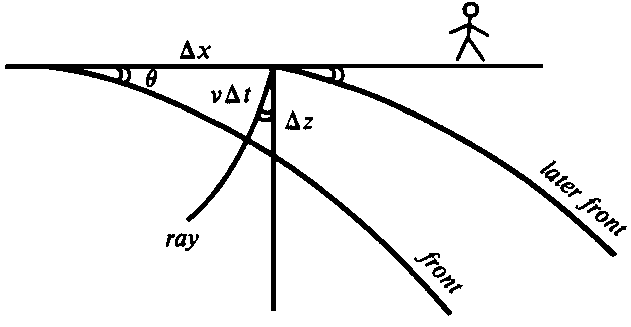
\includegraphics[width=0.65\textwidth]{slnt/fronts}
\caption[fronts]{到达地面的波阵面,观测$dt/dx$可得出比值$dt/dx=(\sin\theta)/v$}
\label{fig:slnt/fronts}
\end{figure}
